\documentclass[12pt]{article}
\usepackage{graphicx}
\usepackage{caption}
\usepackage{subcaption}
\usepackage{tikz}
\usepackage{venndiagram}
\usepackage{venndiagram}
\usepackage{tcolorbox}
\usepackage{listings}
\usepackage{enumitem}
\usepackage{amsmath}
\usepackage{amssymb}
\usepackage{colortbl}
\usepackage{xcolor}
\usepackage[margin=1cm, top=1.5cm, bottom=1.5cm]{geometry}

\tcbuselibrary{breakable}

\title{\textbf{Gráficas y Juegos: Tarea 02}}
\author{Martínez Méndez Ángel Antonio\\Pinzón Chan José Carlos\\Rendón Ávila Jesús Mateo}
\date{\today}

\begin{document}

\maketitle
\begin{center}
\vspace{3cm}
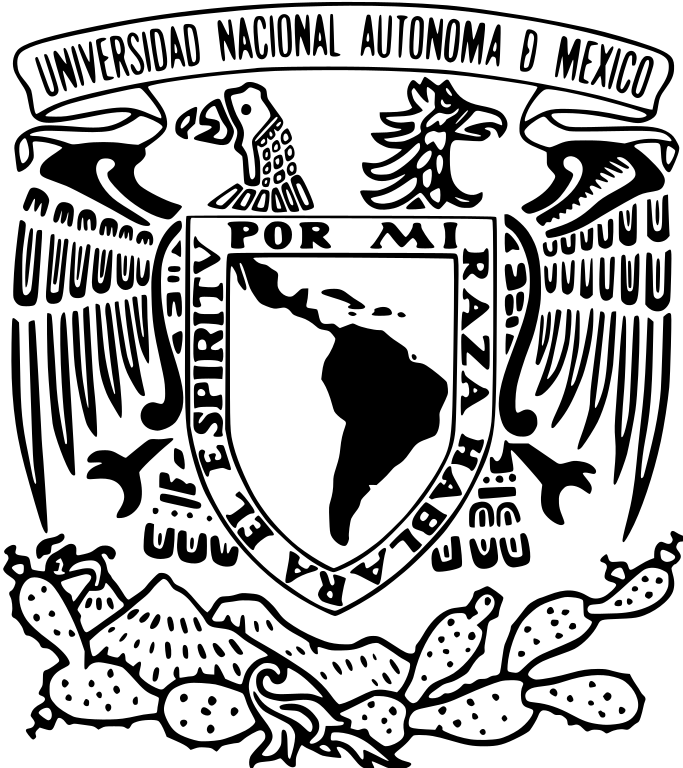
\includegraphics[width=0.195\textwidth]{Escudo.png}
\hspace{0.5cm}
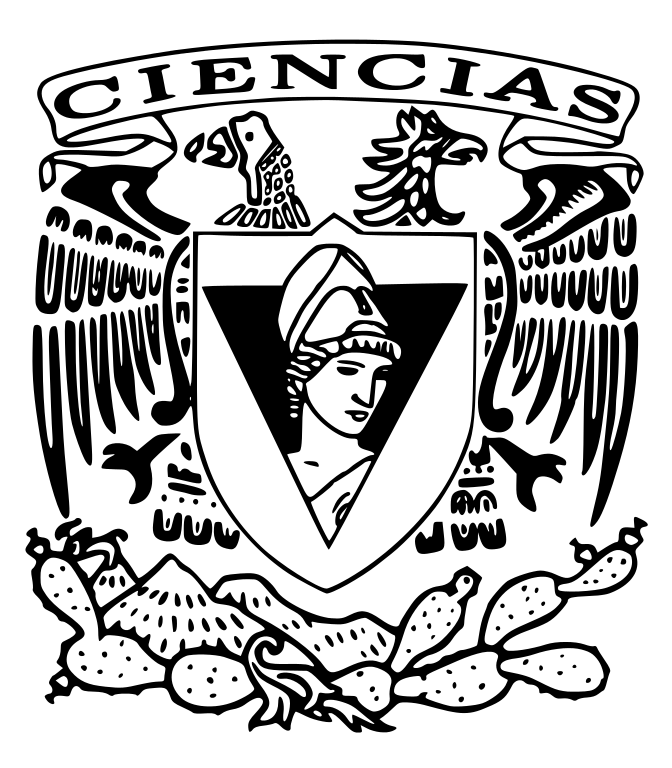
\includegraphics[width=0.2\textwidth]{logo_ciencias.png}
\end{center}
\begin{center}
    \vspace{1cm}
    Universidad Nacional Autónoma de México\\
    Facultad de Ciencias\\
    Profesor: César Hernández Cruz\\
\end{center}

\newpage

%
% Ejercicio 1
%
\textbf{1.} Sea $G$ una gáfica, y recuerde que $c_G$ denota al número de componentes conexas de $G$.
Demuestre que si $e \in E$, entonces $c_G \leq c_{G - e} \leq c_G + 1$.\\

\begin{tcolorbox}[title=\textbf{Hipotesis}, colback=red!15!white, colframe=black!, breakable]
	$G$ es una  gráfica cuyo número de componentes conexas se denota $c_G$ y $e = uv$ es una arista tal que $e \in E_G$
\end{tcolorbox}

\begin{tcolorbox}[title=\textbf{Definiciones}, colback=blue!15!white, colframe=black!, breakable]
    $Def$. A las subgráficas de una gráfica G, máximas por contención con la propiedad de ser conexas, se les llama \textbf{componentes conexas}.
\end{tcolorbox}

Por hipótesis el número de componentes conexas de $G$ es $c_G$. Sabemos que $e \in E_G$ por lo cual $e$ forma parte de alguna componente conexa en G. Como se trata de componentes conexas , entre cualesquiera vértices que pertenezcan a la misma componente conexa que $e$,  existe un $camino$. A partir de este punto se pueden distinguir dos casos generales:\\

Sean $x,y$ dos vértices en la misma componente conexa que $e$.
\begin{enumerate}
 	\item [1)] Existe un $xy-camino$, llamémoslo  $W$, tal que $e$ no forma parte de $W$:\\
	En este caso, como $e$ no forma parte de W entonces al eliminar dicha arista el $xy-camino$ sigue existiendo.
	\item [2)]Existe un $xy-camino$, llamémoslo  $P$, tal que $e$ forma parte de $P$. En este segundo caso es donde divergen dos posibilidades muy 				importantes:
	\begin{enumerate}	
		\item Si entre los vértices $u$ y $v$ existe un $uv-camino$ distinto de \{$u$,$e$,$v$\}, que denotaremos como R, al eliminar la arista $e$ de G, el 	camino P ya no coneca a $x$ con $y$, sin embargo, prevalece un $xy-camino$ descrito del siguiente modo: $xPuRvPy$. En 	consiguiente podemos decir que la grafica sigue siendo conexa y que por lo tanto $c_{G-e}$ = $c_G$.
		
		\item Si entre los vértices $u$ y $v$ el único camino existente es \{$u$,$e$,$v$\}, al eliminar $e$ de G, el camino P deja de 		existir y sucede que $u$ no puede alcanzar a $v$. Como resultado $x$ no puede alcanzar a $y$, oséase, no existe un $xy-camino$; la componente conexa se ha separado.Por el incisio 1), sabemos que todos los caminos en los que $e$ no forma parte se conservan, por lo tanto, en ambas particiones la grafica sigue 	siendo conexa. Asi podemos concluir que $c_{G-e}$ = $c_G$ + 1.
	\end{enumerate}	
\end{enumerate}

A manera de resumen, puede suceder que $c_G$ = $c_{G-e}$, o bien, $c_{G-e}$ = $c_G$ + 1, en otras palabras: $c_G \leq c_{G - e} \leq c_G + 1$.\\

\textit{Nota: Eliminar a la arista \underline{e} no afecta a las componentes conexas a las que \underline{e} no pertenece, es por ello que ignoramos al resto de componentes y nos centramos en la componente de \underline{e}.}


\vspace{1cm}

%
% Ejercicio 2
%
\textbf{2.} Una gráfica es \textit{escindible completa} si su conjunto de vértices admite una partición $(S, K)$
de tal forma que S es un conjunto independiente, $K$ es un clan, y cada vértice en $S$ es
adyacente a cada vértice en $K$. Demuestre que una gráfica es escindible completa si y
sólo si no contiene a $C_4$ ni a $\overline{P_3}$ como subgráfica inducida. (Sugerencia: Un ejercicio de
la tarea anterior puede resultar de utilidad.)
\vspace{1cm}
\begin{tcolorbox}[title=\textbf{Hipótesis}, colback=red!15!white, colframe=black!]
	Una gráfica es \textbf{escindible completa} si y sólo si no contiene a $C_4$ ni a $\overline{P_3}$ como subgráfica inducida.
\end{tcolorbox}
	
\begin{tcolorbox}[title=\textbf{Definiciones}, colback=blue!15!white, colframe=black!]
    $Def$. Una gráfica es \textit{escindible completa} si su conjunto de vértices admite una partición $(S, K)$
de tal forma que S es un conjunto independiente, $K$ es un clan, y cada vértice en $S$ es
adyacente a cada vértice en $K$.\\
	$Def$. Un subconjunto no vacío de vértices de una gráfica es un \textbf{clan} si y sólo si induce una subgráfica completa. Alternativamente, un subconjunto de los vértices de una gráfica G es un clan si y sólo si es un conjunto
independiente en la gráfica complementaria $\overline{G}$.
\end{tcolorbox}

Demostramos por contrapositiva.\\

$\Rightarrow \rfloor$ Sea $G$ una gráfica, tal que $G$ contiene a $\overline{P_3}$ o bien contiene a $C_4$ como subgráfica inducida , entonces G no es escindible completa.   \\

Sea $F$ una gráfica, supongamos que $C_4$ es un subgráfica inducida de $F$. Ahora demostremos que $C_4$ no puede ser escindible completa, esto es, que NO EXISTE una biparticion ($S$,$K$) en $C_4$ tal que $S$ sea un conjunto independiente, $K$ un clan y todo $s \in S$ sea adyacente a todo $k \in K$.\\

Como se trata de una gráfica de 4 vértices y tanto $S$ como $K$ tienen al menos un elemento, eso nos deja tres casos generales para la bipartición ($S$,$K$) en $C_4$.\\

\begin{figure}[h!]
       		 \centering
       		 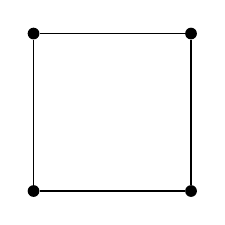
\begin{tikzpicture}[scale=2]
            		\node (a) at (0,0) [circle,fill,inner sep=1.5pt] {};
            		\node (b) at (0,1) [circle,fill,inner sep=1.5pt] {};
            		\node (c) at (1,0) [circle,fill,inner sep=1.5pt] {};
            		\node (d) at (1,1) [circle,fill,inner sep=1.5pt] {};

            		\draw (a) -- (b) (c) -- (d) (b) -- (d) (a) -- (c);

        		\end{tikzpicture}
        		\caption{\scriptsize Representación de $C_4$}
\end{figure}


\begin{enumerate}
 \item[i)] $|S| = |K|$ = 2
 
 Al tratar de elegir vértices para el conjunto S, necesitamos que dichos vértices no sean adyacentes entre si, la única opción es elegir vértices  en esquinas opuestas de $C_4$. Nos queda que $S$ = \{\textcolor{blue}{$v_1,v_3$}\} y $K$ = \{$v_2,v_4$\}.\\
 
 \begin{figure}[h!]
 	\begin{subfigure} {0.6\textwidth}
       		 \centering
       		 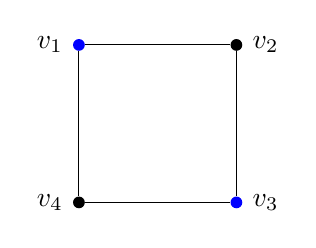
\begin{tikzpicture}[scale=2]
            		\node (a) at (0,0) [circle,fill,inner sep=1.5pt] {};
            		\node [anchor=east] at (a.west) {$\tiny v_4 $}; 
            		\node (b) at (0,1) [circle,fill = blue,inner sep=1.5pt] {};
            		\node [anchor=east] at (b.west) {$\tiny v_1$}; 
            		\node (c) at (1,0) [circle,fill =blue,inner sep=1.5pt] {};
            		\node [anchor=west] at (c.east) {$\tiny v_3$}; 
            		\node (d) at (1,1) [circle,fill,inner sep=1.5pt] {};
            		\node [anchor=west] at (d.east) {$\tiny v_2$}; 

            		\draw (a) -- (b) (c) -- (d) (b) -- (d) (a) -- (c);
            		\draw (a) -- (b) (c) -- (d) (b) -- (d) (a) -- (c);
        		\end{tikzpicture}
        		\caption{\scriptsize Bipartición ($S,K$)}
	\end{subfigure}
	\begin{subfigure} {0.2\textwidth}
       		 \centering
       		 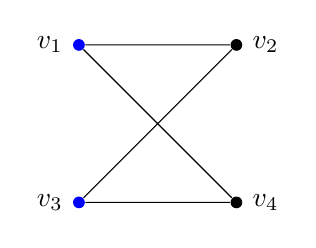
\begin{tikzpicture}[scale=2]
            		\node (a) at (0,0) [circle,fill =blue,inner sep=1.5pt] {};
            		\node [anchor=east] at (a.west) {$\tiny v_3 $}; 
            		\node (b) at (0,1) [circle,fill = blue,inner sep=1.5pt] {};
            		\node [anchor=east] at (b.west) {$\tiny v_1$}; 
            		\node (c) at (1,0) [circle,fill ,inner sep=1.5pt] {};
            		\node [anchor=west] at (c.east) {$\tiny v_4$}; 
            		\node (d) at (1,1) [circle,fill,inner sep=1.5pt] {};
            		\node [anchor=west] at (d.east) {$\tiny v_2$}; 

            		\draw  (b) -- (d) (a) -- (c) (a) -- (d) (b) -- (c);

        		\end{tikzpicture}
        		\caption{\scriptsize Bipartición ($S,K$)}
	\end{subfigure}
\end{figure}
 
 Sin embargo el subconjunto $K$ no es un clan (falta la arista $v_2v_4$). Si intentamos dar cualquier otra partición de estas características para $C_4$ el resultado es análogo, pues (como mencionamos antes) los únicos vértices no adyacentes se encuentran en las esquinas.  \\
 
  \item[ii)] $|S|$ = 1 y $|K|$ = 3
 
 En este otro caso, digamos que $S$ = \{\textcolor{red}{$v_1$}\} y $K$ = \{$v_2,v_3,v_4$\}. Con esta particion, nuevamente $K$ no es un clan (falta la arista $v_2v_4$), y aunque $S$ es independiente, el único vértice en $S$ no es adyacente a todos los vértices en $K$ (falta la arista $v_1v_3$).\\
 
 \begin{figure}[h!]
 	\begin{subfigure} {0.6\textwidth}
       		 \centering
       		 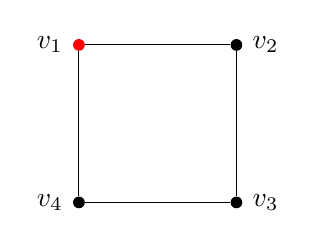
\begin{tikzpicture}[scale=2]
            		\node (a) at (0,0) [circle,fill,inner sep=1.5pt] {};
            		\node [anchor=east] at (a.west) {$\tiny v_4 $}; 
            		\node (b) at (0,1) [circle,fill,inner sep=1.5pt, color = red] {};
            		\node [anchor=east] at (b.west) {$\tiny v_1$}; 
            		\node (c) at (1,0) [circle,fill,inner sep=1.5pt] {};
            		\node [anchor=west] at (c.east) {$\tiny v_3$}; 
            		\node (d) at (1,1) [circle,fill,inner sep=1.5pt] {};
            		\node [anchor=west] at (d.east) {$\tiny v_2$}; 

            		\draw (a) -- (b) (c) -- (d) (b) -- (d) (a) -- (c);
        		\end{tikzpicture}
        		\caption{\scriptsize Bipartición ($S,K$)}
	\end{subfigure}
	\begin{subfigure} {0.2\textwidth}
       		 \centering
       		 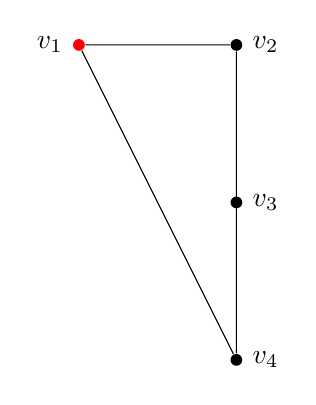
\begin{tikzpicture}[scale=2]
            		\node (a) at (1,0) [circle,fill,inner sep=1.5pt] {};
            		\node [anchor=west] at (a.east) {$\tiny v_4 $}; 
            		\node (b) at (1,2) [circle,fill,inner sep=1.5pt] {};
            		\node [anchor=west] at (b.east) {$\tiny v_2$}; 
            		\node (c) at (1,1) [circle,fill,inner sep=1.5pt] {};
            		\node [anchor=west] at (c.east) {$\tiny v_3$}; 
            		\node (d) at (0,2) [circle,fill = red,inner sep=1.5pt] {};
            		\node [anchor=east] at (d.west) {$\tiny v_1$}; 

            		\draw  (b) -- (d) (a) -- (c) (a) -- (d) (b) -- (a);

        		\end{tikzpicture}
        		\caption{\scriptsize Bipartición ($S,K$)}
	\end{subfigure}
\end{figure}

\begin{center}
Este resultado es análogo, no importa que vértice en $C_4$ elijamos para el subconjunto $S$.\\
\end{center}


	\item[iii)] $|S|$ = 3 y $|K|$ = 1
	
	Esta partición en $C_4$ es imposible ya que cualesquiera 3 vértices que elijamos para $S$, al menos dos son adyacentes (no se cumple que $S$ sea un conjunto independiente).\\
	
	\begin{figure}[h!]
       		 \centering
       		 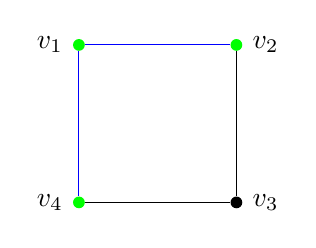
\begin{tikzpicture}[scale=2]
            		\node (a) at (0,0) [circle,fill,inner sep=1.5pt,color = green] {};
            		\node [anchor=east] at (a.west) {$\tiny v_4 $}; 
            		\node (b) at (0,1) [circle,fill,inner sep=1.5pt,color = green] {};
            		\node [anchor=east] at (b.west) {$\tiny v_1$}; 
            		\node (c) at (1,0) [circle,fill,inner sep=1.5pt] {};
            		\node [anchor=west] at (c.east) {$\tiny v_3$}; 
            		\node (d) at (1,1) [circle,fill,inner sep=1.5pt,color = green] {};
            		\node [anchor=west] at (d.east) {$\tiny v_2$}; 

            		\draw[blue](a) -- (b)  (b) -- (d) ;
            		\draw (a) -- (c) (c) -- (d);

        		\end{tikzpicture}
        		\caption{\scriptsize Problema del caso iii)}
	\end{figure}
\end{enumerate}

$\therefore$ Si $F$ contiene a $C_4$ como subgráfica inducida, entonces $F$ no es escindible completa. Note que si tuvieramos la gráfica $F$, como $F$ contiene a $C_4$, entonces al intentar dar una biparticion ($S$,$K$) para $F$, experimentaríamos los problemas vistos anteriormente, derivados del $C_4$ en su interior.\\


Supongamos ahora que $\overline{P_3}$ es una subgráfica inducida de $F$, de manera similar a lo hecho en $C_4$, intentemos mostrar que NO EXISTE una biparticion ($S$,$K$) en $\overline{P_3}$ tal que $S$ sea un conjunto independiente, $K$ un clan y todo $s \in S$ sea adyacente a todo $k \in K$. Comenzemos rápidamente con los casos para dicha particion:\\

\begin{figure}[h!]
       		 \centering
       		 \begin{tikzpicture}[scale=2]
            		\node (a) at (0,0) [circle,fill,inner sep= 1.5pt] {};
            		\node[anchor=east] at (a.west) {$\tiny v_2 $}; 
            		\node (b) at (0.5,1) [circle,fill,inner sep= 1.5pt] {};
            		\node[anchor=south] at (b.north) {$\tiny v_1 $}; 
            		\node (c) at (1,0) [circle,fill,inner sep= 1.5pt] {};
            		\node[anchor=west] at (c.east) {$\tiny v_3 $}; 

            		\draw (a) -- (c);

        		\end{tikzpicture}
        		\caption{\scriptsize Representación de $\overline{P_3}$}
\end{figure}

\begin{enumerate}
	\item[i)] $|S|$ = 2 y $|K|$ = 1\\
	
	Necesitamos que los vértices en $S$ sean no adyacentes, asi que diremos que $S$ = \{\textcolor{red}{$v_1,v_2$}\} y $K$ = \{$v_3$\}. El subconjunto $S$ cumple con ser independiente, además $K$ es un clan (pues $|K|$ = 1), no obstante , el vértice $v_1 \in S$ no es adyacente al vértice $v_3 \in K$. Al elegir al vértice $v_3$ en lugar de $v_2$ esto sigue ocurriendo.\\
	
\begin{figure}[h!]
 	\begin{subfigure} {0.6\textwidth}
       		 \centering
       		 \begin{tikzpicture}[scale=2]
            		\node (a) at (0,0) [circle,fill = red,inner sep= 1.5pt] {};
            		\node[anchor=east] at (a.west) {$\tiny v_2 $}; 
            		\node (b) at (0.5,1) [circle,fill =red,inner sep= 1.5pt] {};
            		\node[anchor=south] at (b.north) {$\tiny v_1 $}; 
            		\node (c) at (1,0) [circle,fill,inner sep= 1.5pt] {};
            		\node[anchor=west] at (c.east) {$\tiny v_3 $}; 

            		\draw (a) -- (c);
        		\end{tikzpicture}
        		\caption{\scriptsize Bipartición ($S,K$)}
	\end{subfigure}
	\begin{subfigure} {0.2\textwidth}
       		 \centering
       		 \begin{tikzpicture}[scale=2]
            		\node (a) at (0,0) [circle,fill = red,inner sep=1.5pt,text=white] {};
            		\node[anchor=east] at (a.west) {$\tiny v_2 $}; 
            		\node (b) at (0,1) [circle,fill =red,inner sep=1.5pt,text=white] {};
            		\node[anchor=east] at (b.west) {$\tiny v_1 $}; 
            		\node (c) at (1,0.5) [circle,fill =black,inner sep=1.5pt,text=white] {};
            		\node[anchor=west] at (c.east) {$\tiny v_3 $}; 


            		\draw  (a) -- (c);

        		\end{tikzpicture}
        		\caption{\scriptsize Bipartición ($S,K$)}
	\end{subfigure}
\end{figure}

	

	\item[ii)] $|S|$ = 1 y $|K|$ = 2\\

	En este caso nos vemos obligados a decir que $K$ = \{$v_2,v_3$\} pues son los únicos 2 vértices adyacentes en $\overline{P_3}$; naturalmente $S$ = \{\textcolor{blue}{$v_1$}\}.\\

\begin{figure}[h!]
 	\begin{subfigure} {0.6\textwidth}
       		 \centering
       		 \begin{tikzpicture}[scale=2]
            		\node (a) at (0,0) [circle,fill,inner sep= 1.5pt] {};
            		\node[anchor=east] at (a.west) {$\tiny v_2 $}; 
            		\node (b) at (0.5,1) [circle,fill =blue,inner sep= 1.5pt] {};
            		\node[anchor=south] at (b.north) {$\tiny v_1 $}; 
            		\node (c) at (1,0) [circle,fill,inner sep= 1.5pt] {};
            		\node[anchor=west] at (c.east) {$\tiny v_3 $}; 

            		\draw (a) -- (c);
        		\end{tikzpicture}
        		\caption{\scriptsize Bipartición ($S,K$)}
	\end{subfigure}
	\begin{subfigure} {0.2\textwidth}
       		 \centering
       		 \begin{tikzpicture}[scale=2]
            		\node (a) at (1,0) [circle,fill,inner sep=1.5pt,text=white] {};
            		\node[anchor=east] at (a.west) {$\tiny v_2 $}; 
            		\node (b) at (0,0.5) [circle,fill =blue,inner sep=1.5pt,text=white] {};
            		\node[anchor=east] at (b.west) {$\tiny v_1 $}; 
            		\node (c) at (1,1) [circle,fill =black,inner sep=1.5pt,text=white] {};
            		\node[anchor=west] at (c.east) {$\tiny v_3 $}; 


            		\draw  (a) -- (c);

        		\end{tikzpicture}
        		\caption{\scriptsize Bipartición ($S,K$)}
	\end{subfigure}
\end{figure}
	Observe que K cumple con ser un clan nuevamente, pero $v_1 \in S$ no es adyacente a ninguno de los 2 vértices en $K$. Otra vez tenemos que $\overline{P_3}$ no puede darnos una bipartición ($S,K$) donde todo vértice en $S$ sea adyacente a todo vértice en $K$.
	
\end{enumerate}
$\therefore$ Si $F$ contiene a $\overline{P_3}$, entonces $F$ no es escindible completa, pues $\overline{P_3}$ no cumple con la definición de ser escindible completa. No importa si existe una bipartición ($S,K$) para el resto de vértices de $F$, al intentar inlcuir en dicha bipartición a los vértices de $\overline{P_3}$, automáticamente la definición deja de cumplirse.\\

$\therefore$ Si $G$ es una gráfica, tal que $G$ contiene a $C_4$ o bien contiene a $\overline{P_3}$ como subgráfica inducida , entonces G no es escindible completa.\\

$\Leftarrow \rfloor$ Sea $G$ una gráfica, si $G$ es no es escindible completa, entonces $G$ contiene a $C_4$ o a $\overline{P_3}$ como subgráfica inducida.\\

Una gráfica $F$ no es escindible completa, si al dar una bipartición ($S,K$), se cumple al menos una de las siguientes afirmaciones:\\

\begin{enumerate}
	\item $S$ no es independiente.
	\item $K$ no es un clan.
	\item Al menos un vértice en $S$ no es adyacente a algun vértice en $K$.
\end{enumerate}

Existen 6 posibles casos (este número se obtiene de las permutaciones de las 3 afirmaciones anteriores) en los que una gráfica resulta no ser escindible completa. Analizemos si en cada uno de ellos podemos inferir la existencia de $\overline{P_3}$ o de $C_4$.\\

Cabe resaltar que daremos por hecho el resto de propiedades de la definición de escindible completa, por ejemplo, en el caso i) decimos que $S$ no es independiente,es decir, suponemos que el resto de propiedades se cumplen: $K$ es un clan y que todo $s \in S$ es adyacente a todo $k \in K$.\\
\begin{enumerate}
	\item[i)]$S$ no es independiente
	
	Al $S$ no ser independiente, podemos suponer la existencia de una arista $ss'$ tal que $s,s' \in S$. También podemos afirmar que existe una $sk_1$ y $s'k_2$ aristas. Además,como $K$ es un clan, entonces la arista $k_1k_2$ existe.\\
	
	$\therefore$ Existe un ciclo $C$ de longitud 4, tal que $C$ = \{$s,k_1,k_2,s',s$\}.\\
	
	\item[ii)]$K$ no es un clan.
	
	Como $K$ no es un clan, al menos entre 2 vértices $k_i,k_j \in K$ no existe un arista. Llamemos a estos vértices $k_1$ y $k_2$.\\
	
	Sean $s_1,s_2 \in S$; entonces existyen las aristas $s_1k_1,s_1k_2,s_2k_1,s_2k_2$.\\
	
	$\therefore$ Existe un ciclo $C$ de longitud 4, donde $C$ = \{$s_1,k_1,s_2,k_2,s_1$\}.\\
	
	\item[iii)]Al menos un vértice en $S$ no es adyacente a algun vértice en $K$.
	
	Sean $s_1,s_2 \in S$ y $k_1,k_2 \in K$, diremos (por hipótesis) que $s_2$ no es adyacente a $k_1$. Entonces por lo menos tenemos las siguientes aristas: $s_1k_1,s_1k_2,s_2k_1,k_1k_2$.\\
	
	Si eliminamos al vértice $k_2$, entonces de las aristas antes mencionadas, sólo se conserva la arista $s_1k_1$. Observe que $s_1$ y $k_1$ son adyacentes pero $s_2$ no es adyacente a nadie.\\
	
	$\therefore$ $\overline{P_3}$ es una subgráfica inducida de $F$.\\
	
	\item[iv)]$S$ no es independiente y $K$ no es un clan.
	
	En el peor de los casos la gráfica de $S$ es completa y la de $K$ es vacía. Pero si es así, entonces basta con redefinir quien es $S$ y quien es $K$ y resulta que $F$ es escindible completa.Si ignoramos este caso "extremo", nos topamos con que entonces podemos eliminar vértices $s_i \in S$ hasta que $S$ sea independiente. Análogamente, podríamos eliminar vértices $k_j \in K$ hasta que $K$ sea un clan.\\
	
	Bajo esta lógica, si eliminamos \textbf{solamente} vértices en $S$, hasta que $S$ sea independiente, podemos aplicar el caso ii) y decir que $F$ tiene a $C_4$ como subgráfica inducida. Si eliminamos \textbf{solamente} vértices en $K$, hasta que $K$ sea un clan, podemos aplicar el caso i) y decir que $F$ tiene a $C_4$ como subgráfica inducida.\\
	
	$\therefore$ $F$ tiene a $C_4$ como subgráfica inducida.\\
	
	\item[v)]$S$ no es independiente y al menos un vértice en $S$ no es adyacente a algun vértice en $K$.\\
	
	En el caso en el cual la gráfica de $S$ sea completa y $\forall s_i \in S$, $s_i$ no es adyacente a ningun $k_j \in K$. Podemos eliminar vértices en $S$ hasta dejar únicamente 2, eliminar vértices en $K$ hasta dejar uno y viceversa. Nos queda entonces que $\overline{P_3}$ es subgráfica de $F$.\\
	
	En cualquier otro caso la gráfica de $S$ no es completa y existe al menos un $s_i \in S$ tal que $s_i$ no es adyacente a algun $k_j \in K$. Nombremos a este vértice $s_0$. Al eliminar todos los vértices en $S$ excepto a $s_0$, $S$ se vuelve independiente, y podemos aplicar el caso iii), que nos dice que $\overline{P_3}$ es una subgráfica inducida de $F$.\\
	
	$\therefore$ $F$ tiene a  $\overline{P_3}$ como subgráfica inducida.\\
	
	\item[vi)]$S$ no es independiente, $K$ no es un clan y al menos un vértice en $S$ no es adyacente a algun vértice en $K$.\\
	
	En el caso más interesante, $S$ es completa y $K$ es vacía, renombrando quien es $S$ y quien es $K$ podemos aplicar el caso iii). En otras circunstancias, siempre ocurre que podemos hacer que $S$ sea independiente o bien que $K$ sea un clan. Dependiendo de las circunstancias podremos aplicar los casos iv) o v).\\
	
\end{enumerate}

	$\therefore$ $F$ contiene a $C_4$ o a $\overline{P_3}$ como subgráfica inducida.\\

	$\therefore$ Si $G$ no es escindible completa, entonces contiene a $C_4$ o $\overline{P_3}$ a  como subgráfica inducida.\\
	
	$\therefore$ Una gráfica es \textbf{escindible completa} si y sólo si no contiene a $C_4$ ni a $\overline{P_3}$ como subgráfica inducida.\\
\vspace{1cm}

%
% Ejercicio 3
%
\textbf{3}.

\begin{enumerate}[label=\alph*)]

    \item Demuestre que si $\mid E \mid >$ \( \binom{|V|-1}{2} \), entonces $G$ es conexa.
    \begin{tcolorbox}[title=\textbf{Definiciones}, colback=blue!15!white, colframe=black!]
        $Def.$ \textbf{Gráfica conexa}: G es conexa si para todos $u, v \in V$  existe un $uv$-camino.\\

        $Def.$ \textbf{Coeficiente binomial}: Denotado por \( \binom{n}{2} \), representa el número de maneras 
        de elegir subconjuntos de tamaño $2$ a partir de un conjunto de $n$ elementos.
    
    \end{tcolorbox}
    \begin{tcolorbox}[title=\textbf{Hipotesis}, colback=red!15!white, colframe=black!]
        $Hip.$ Sea $G$ una gráfica que cumple $\mid E \mid >$ \( \binom{|V|-1}{2} \)

    \end{tcolorbox}

    Notemos que las gráficas que cumplen con nuestra hipótesis, empiezan justo después del caso donde:

    \begin{center}
        $\mid E \mid$ = \( \binom{|V|-1}{2} \)
    \end{center}

    Es decir, desde el caso en el que nuestras gráficas son inconexas. Esto es debido a que este tipo particular de 
    gráficas, dada un número $n$ arbitrario de vertices, donde $n > 3$, tienen como subgráfica inducida a un $K_{n-1} \cup v$ 
    donde, $v$ representa a un vertice aislado.\\

    Representemos esta inconexidad suponiendo que en una gráfica $H$, cumple que
    $\mid E_H \mid$ = \( \binom{|V|-1}{2} \) donde podemos hacer un partición $(X,Y)$ en $V_H$ donde en $X$ existe un $ux$-camino
    camino $uWx$, donde $v, x \in K_{n-1}$ y además, $y \in Y$ que es nuestro vertice aislado.\\

    Como es evidente, para que este tipo de gráficas tenga un $uv$-camino, particularmente que exista 
    un $uy$-camino en $H$, i.e. que sea conexa, es necesario que en las particiones de estas gráficas 
    $(X,Y)$ sean adyacentes, dicho de otro modo:

    \begin{center}
        $\mid E \mid >$ \( \binom{|V|-1}{2} \)
    \end{center}

    O bien:

    \begin{center}
        \( \binom{|V|-1}{2} \) + 1 $>$ \( \binom{|V|-1}{2} \)
    \end{center}

    Donde debe existir una aristas más en nuestra gráfica $G$ para que sea conexa, justo lo que es nuestra 
    hipótesis. Lo que quiere decir que las gráficas que cumplan:

    \begin{center}
        $\mid E \mid >$ \( \binom{|V|-1}{2} \)
    \end{center}

    En efecto, son conexas, pues existe un uv-camino para cada $u, v \in V$.


    \item Para cada $n > 3$ encuentre una gráfica inconexa de orden $n$ con $\mid E \mid$ = \( \binom{n-1}{2} \)\\

    Dibujando los gŕaficas para $n = 4, n = 5, n = 6$ y $n = 7$\\

    \begin{figure}[h!]
        \centering
        \begin{minipage}{0.2\textwidth}
            \centering
            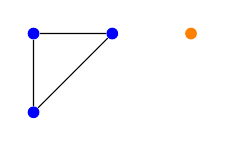
\begin{tikzpicture}[scale=1]
                \node (a) at (0,0) [circle,fill,inner sep=1.5pt,color=blue] {};
                \node (b) at (0,1) [circle,fill,inner sep=1.5pt,color=blue] {};
                \node (c) at (1,1) [circle,fill,inner sep=1.5pt,color=blue] {};
                \node (d) at (2,1) [circle,fill,inner sep=1.5pt,color=orange] {};

                \draw (a) -- (b) (b) -- (c) (a) -- (c);
    
            \end{tikzpicture}
            \caption{\scriptsize Representación de una gráfica con una subgráfica $3$-regular de 4 vertices, uno aislado, con 3 aristas }
        \end{minipage}
        \hspace{0.20\textwidth}
        \begin{minipage}{0.2\textwidth}
            \centering
            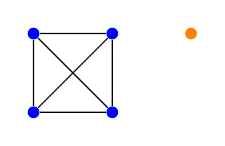
\begin{tikzpicture}[scale=1]
                \node (a) at (0,0) [circle,fill,inner sep=1.5pt,color=blue] {};
                \node (b) at (0,1) [circle,fill,inner sep=1.5pt,color=blue] {};
                \node (c) at (1,0) [circle,fill,inner sep=1.5pt,color=blue] {};
                \node (d) at (1,1) [circle,fill,inner sep=1.5pt,color=blue] {};
                \node (e) at (2,1) [circle,fill,inner sep=1.5pt,color=orange] {};

                \draw (a) -- (b) (b) -- (d) (d) -- (c) (c) -- (a) (a) -- (d) (b) -- (c);
    
            \end{tikzpicture}
            \caption{\scriptsize Representación de una gráfica con una subgráfica $4$-regular de 5 vertices, uno aislado, con 6 aristas}
        \end{minipage}
        \hspace{0.20\textwidth}
        \begin{minipage}{0.2\textwidth}
            \centering
            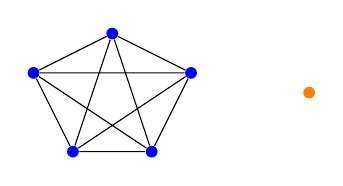
\begin{tikzpicture}[scale=1]
                \node (a) at (0,0) [circle,fill,inner sep=1.5pt,color=blue] {};
                \node (b) at (1,0) [circle,fill,inner sep=1.5pt,color=blue] {};
                \node (c) at (1.5,1) [circle,fill,inner sep=1.5pt,color=blue] {};
                \node (d) at (0.5,1.5) [circle,fill,inner sep=1.5pt,color=blue] {};
                \node (e) at (-0.5,1) [circle,fill,inner sep=1.5pt,color=blue] {};
                \node (f) at (3,0.75) [circle,fill,inner sep=1.5pt,color=orange] {};

                \draw (a) -- (b) (a) -- (c) (a) -- (d) (a) -- (e) (b) -- (c) (b) -- (d) (b) -- (e) 
                (c) -- (d) (c) -- (e) (d) -- (e);

                
            \end{tikzpicture}
            \caption{\scriptsize Representación de una gráfica con una subgráfica $5$-regular de 6 vertices, uno aislado, con 10 aristas}
        \end{minipage}
        \hspace{0.20\textwidth}
        \begin{minipage}{0.2\textwidth}
            \centering
            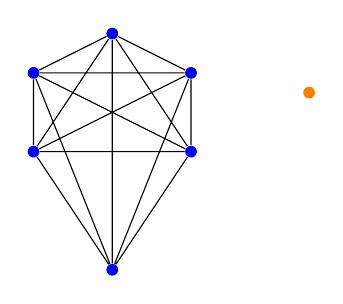
\begin{tikzpicture}[scale=1]
                \node (a) at (-0.5,0) [circle,fill,inner sep=1.5pt,color=blue] {};
                \node (b) at (1.5,0) [circle,fill,inner sep=1.5pt,color=blue] {};
                \node (c) at (1.5,1) [circle,fill,inner sep=1.5pt,color=blue] {};
                \node (d) at (0.5,1.5) [circle,fill,inner sep=1.5pt,color=blue] {};
                \node (e) at (-0.5,1) [circle,fill,inner sep=1.5pt,color=blue] {};
                \node (f) at (0.5,-1.5) [circle,fill,inner sep=1.5pt,color=blue] {};
                \node (g) at (3,0.75) [circle,fill,inner sep=1.5pt,color=orange] {};
                
                \draw (a) -- (b) (a) -- (c) (a) -- (d) (a) -- (e) (a) -- (f) (b) -- (c) 
                (b) -- (d) (b) -- (e) (b) -- (f) (c) -- (d) (c) -- (e) (c) -- (f) (d) -- (e)
                (d) -- (f) (e) -- (f);

            \end{tikzpicture}
            \caption{\scriptsize Representación de una gráfica con una subgráfica $6$-regular de 7 vertices, uno aislado, con 15 aristas}
        \end{minipage}
    \end{figure}
    \newpage

    Notemos que las gráficas obtenidas tienen la particularidad de tener inducidas en ellas, como subgráfica, a un $K_{n-1} \cup v$ donde, $v$ 
    representa a un vertice aislado dado un $n$ arbitrario que representa justamente $|V| = n$. Y cumple 
    con la condición de que $\mid E \mid = \binom{n-1}{2} = \frac{(n-1)(n-2)}{2}$.

    
    
\end{enumerate}

\vspace{1cm}
%
% Ejercicio 4
%
\textbf{4.}
\begin{enumerate}[label=\alph*)]

    \item Demuestre que si $\delta >  \left( \left\lfloor \frac{|V|}{2} \right\rfloor - 1 \right)$, entonces $G$ es conexa.
    \begin{tcolorbox}[title=\textbf{Hipotesis}, colback=red!15!white, colframe=black!]
        El grado minimo $\delta$ de $G$ es mayor a $\left( \left\lfloor \frac{|V|}{2} \right\rfloor - 1 \right)$.
    \end{tcolorbox}

        Sea $G$ una gráfica cuyo grado minimo es $\delta > \left( \left\lfloor \frac{|V|}{2} \right\rfloor - 1 \right)$, entonces
        podemos decir quev $\delta \geq  \left\lfloor \frac{|V|}{2} \right\rfloor - 1 + 1$, es decir:

        \begin{center}
        $\delta \geq  \left\lfloor \frac{|V|}{2} \right\rfloor$
        \end{center}

        Si $S$ es un subconjunto de $ V(G)$ que satisface $|S| = |V| - 2$ y $u$, $v$ dos vértices
        que pertenecen a $V(G)$ y no pertenecen a $S$.\\

        Como sabemos que $u, v \notin S$. Si es que $u$ es adyacente 
        a $\frac{|S|}{2}$ elementos $s \in S$ y $v$ es adyacente a $\frac{|S|}{2}$ elementos $s' \in S$, es decir,
        $u$ es adyacente a $\frac{|V| - 2}{2}$ elementos $s \in S$ y $v$ es adyacente a
        $\frac{|V| - 2}{2}$ elementos $s' \in S$. Con lo anterior podemos decir que $u$ es adyacente a los elementos del 
        subconjunto de $S$ $\{s_0, s_1, s_2, \dots, s_n\}$, mientras que $v$ es adyacente a los elementosdel subconjunto de $S$
        $\{s'_0, s'_1, s'_2, \dots, s'_n\}$\\

        Como por hipotesis sabemos que $d(u), d(v) \geq \left\lfloor \frac{|V|}{2} \right\rfloor$, entonces cuando
        $|V|$ es impar debe haber un $s^{\ast}$ en $S$ tal que $s_n = s^{\ast} = s'_n$.
        Mientras que cuando $|V|$ es par, existe otro $s^{\ast \ast}$ que cumple $s_i = s^{\ast \ast} = s'_i$ a los cuales $u$ y $v$ son adyacentes.
        Por lo que podemos grantizar una $uv$- trayectoria $P$:
        
        \begin{center}
            $P = (u, s_n = s^{\ast} = s'_n, v)$ cuando $|V|$ es par e impar y\\

            $P' = (u, s_n = s^{\ast \ast} = s'_n, v)$, cuando $|V|$ es par
        \end{center}

        para cada $u, v \in V(G)$. Por lo tanto $G$ es conexa.\\
        $\hfill \blacksquare$ 
        \begin{figure}[h!]

        \centering
        \begin{minipage}{0.2\textwidth}
            \centering
        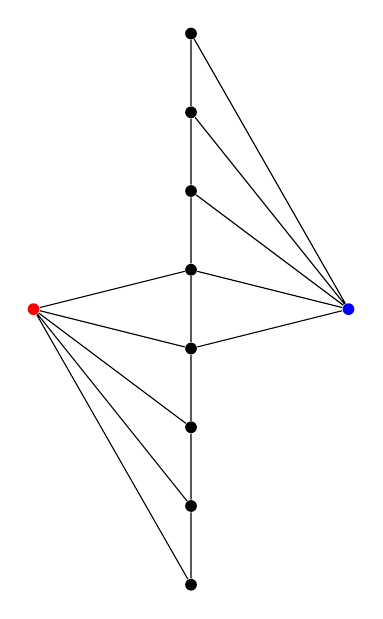
\begin{tikzpicture}[scale=1]
            \node (a) at (2,0) [circle,fill,inner sep=1.5pt] {};
            \node (b) at (2,1) [circle,fill,inner sep=1.5pt] {};
            \node (c) at (2,2) [circle,fill,inner sep=1.5pt] {};
            \node (d) at (2,3) [circle,fill,inner sep=1.5pt] {};
            \node (e) at (2,4) [circle,fill,inner sep=1.5pt] {};
            \node (f) at (2,5) [circle,fill,inner sep=1.5pt] {};
            \node (g) at (2,6) [circle,fill,inner sep=1.5pt] {};
            \node (h) at (2,7) [circle,fill,inner sep=1.5pt] {};

            \node (u) at (0,3.5) [circle,fill,inner sep=1.5pt, color=red] {};
            \node (v) at (4,3.5) [circle,fill,inner sep=1.5pt, color=blue] {};
            \draw (u) -- (a) (u) -- (b) (u) -- (c) (u) -- (d) (u) -- (e) (v) -- (e) (v) -- (f) (v) -- (g) (v) -- (h) (v) -- (d)
            (a) -- (b) (b) -- (c) (c) -- (d) (d) -- (e) (e) -- (f) (f) -- (g) (g) -- (h);
        \end{tikzpicture}
            \caption{\scriptsize Representación de $G$ cuando $|V|$ es par, suponiendo que en la columna central (negra) son adaycentes cualesqueira 2 vértices.}

       \end{minipage}
        \hspace{0.1\textwidth}
        \begin{minipage}{0.2\textwidth}
            \centering
        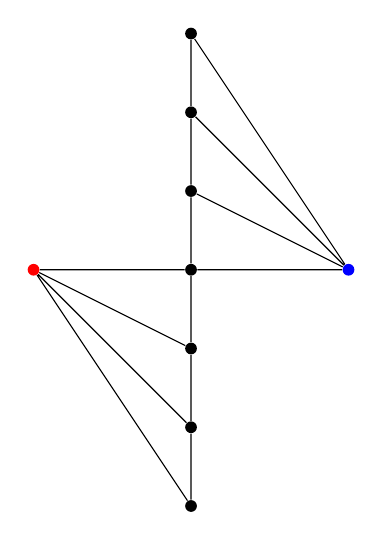
\begin{tikzpicture}[scale=1]
            \node (a) at (2,0) [circle,fill,inner sep=1.5pt] {};
            \node (b) at (2,1) [circle,fill,inner sep=1.5pt] {};
            \node (c) at (2,2) [circle,fill,inner sep=1.5pt] {};
            \node (d) at (2,3) [circle,fill,inner sep=1.5pt] {};
            \node (e) at (2,4) [circle,fill,inner sep=1.5pt] {};
            \node (f) at (2,5) [circle,fill,inner sep=1.5pt] {};
            \node (g) at (2,6) [circle,fill,inner sep=1.5pt] {};

            \node (u) at (0,3) [circle,fill,inner sep=1.5pt, color=red] {};
            \node (v) at (4,3) [circle,fill,inner sep=1.5pt, color=blue] {};
            \draw (u) -- (a) (u) -- (b) (u) -- (c) (u) -- (d) (v) -- (e) (v) -- (f) (v) -- (g)  (v) -- (d)
            (a) -- (b) (b) -- (c) (c) -- (d) (d) -- (e) (e) -- (f) (f) -- (g);

        \end{tikzpicture}
            \caption{\scriptsize Representación de $G$ cuando $|V|$ es impar, suponiendo que en la columna central (negra) son adyacentes cualesquiera 2 vertices.}
       \end{minipage}

        \end{figure}
        

    \item Para $|V|$ par encuentre una gráfica $\left( \left\lfloor \frac{|V|}{2} \right\rfloor - 1 \right)$-regular e inconexa.\\

        Como podemos ver de dibujar las gráficas para $|V| = 2, |V| = 4, |V| = 6$ y $|V| = 8$\\

    
%Primera fila de graficas
\begin{figure}[h!]
    \centering
    \begin{minipage}{0.2\textwidth}
        \centering
        
\begin{tikzpicture}[scale=1]
            \node (a) at (0,0) [circle,fill,inner sep=1.5pt,color=red] {};
            \node (b) at (0,1) [circle,fill,inner sep=1.5pt] {};

        \end{tikzpicture}
        \caption{\scriptsize Representación de una gráfica $0$-regular de 2 vértices}
    \end{minipage}
    \hspace{0.015\textwidth}
    \begin{minipage}{0.2\textwidth}
        \centering
        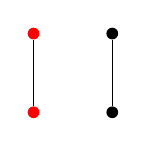
\begin{tikzpicture}[scale=1]
            \node (a) at (0,0) [circle,fill,inner sep=1.5pt,color=red] {};
            \node (b) at (0,1) [circle,fill,inner sep=1.5pt,color=red] {};
            \node (c) at (1,0) [circle,fill,inner sep=1.5pt] {};
            \node (d) at (1,1) [circle,fill,inner sep=1.5pt] {};

            \draw (a) -- (b) (c) -- (d);

        \end{tikzpicture}
        \caption{\scriptsize Representación de una gráfica $1$-regular de 4 vértices}
    \end{minipage}
    \hspace{0.015\textwidth}
    \begin{minipage}{0.2\textwidth}
        \centering
        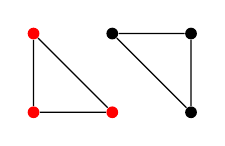
\begin{tikzpicture}[scale=1]
            \node (a) at (0,0) [circle,fill,inner sep=1.5pt,color=red] {};
            \node (b) at (0,1) [circle,fill,inner sep=1.5pt,color=red] {};
            \node (c) at (1,0) [circle,fill,inner sep=1.5pt,color=red] {};
            \node (d) at (1,1) [circle,fill,inner sep=1.5pt] {};
            \node (e) at (2,0) [circle,fill,inner sep=1.5pt] {};
            \node (f) at (2,1) [circle,fill,inner sep=1.5pt] {};


            \draw (a) -- (b) (a) -- (c) (b) -- (c) (d) -- (e) (d) -- (f) (e) -- (f);

        \end{tikzpicture}
        \caption{\scriptsize Representación de una gráfica $2$-regular de 6 vértices}
    \end{minipage}
    \hspace{0.015\textwidth}
    \begin{minipage}{0.2\textwidth}
        \centering
        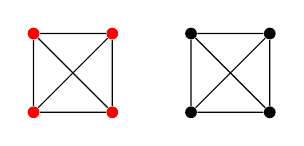
\begin{tikzpicture}[scale=1]
            \node (a) at (0,0) [circle,fill,inner sep=1.5pt,color=red] {};
            \node (b) at (0,1) [circle,fill,inner sep=1.5pt,color=red] {};
            \node (c) at (1,0) [circle,fill,inner sep=1.5pt,color=red] {};
            \node (d) at (1,1) [circle,fill,inner sep=1.5pt,color=red] {};
            \node (e) at (2,0) [circle,fill,inner sep=1.5pt] {};
            \node (f) at (2,1) [circle,fill,inner sep=1.5pt] {};
            \node (g) at (3,0) [circle,fill,inner sep=1.5pt] {};
            \node (h) at (3,1) [circle,fill,inner sep=1.5pt] {};


            \draw (a) -- (b) (a) -- (c) (b) -- (d) (d) -- (c) (a) -- (d) (b) -- (c) (e) -- (f) (f) -- (g) (g) -- (h) (e) -- (g) (f) -- (h) (e) -- (h);

        \end{tikzpicture}
        \caption{\scriptsize Representación de una gráfica $3$-regular de 6 vértices}
    \end{minipage}
\end{figure}

    Podemos decir que las gráficas que representan la condición son las $2k_n$ con $n \geq 1$ y $n \in \mathbb{N}$.

\end{enumerate}

\vspace{1cm}

%
% Ejercicio 5
%
\textbf{5.} Demuestre que si $D$ no tiene lazos y $\delta^+ \geq 1$, entonces $D$ contiene un ciclo dirigido de longitud 
al menos $\delta^+ + 1$.\\

\begin{tcolorbox}[title=\textbf{Hipotesis}, colback=red!15!white, colframe=black!]
    Sabemos que $D$ no tiene lazos y ademas $\delta^{+} \geq 1$.
\end{tcolorbox}
$P.D$ La gráfica $D$ contiene un cilco dirigido de longitud al menos $\delta^{+} + 1$

Sea $D$ una gráfica dirgida que conntiene una trayecttoria dirigida máxima $P$ tal que:
\begin{center}
    $P = (d_1, e_1, d_2, e_2, \dots,d_{k-1}, e_{k - 1}, d_k)$
\end{center}
Como sabemos que P es de longitud máxima y además el exgrado minimo de $D$ es mayor o igual a 1, entonces el vértice $d_k$ tiene 
una arísta saleinte $e_k$ que, por ser $P$ de longitud máxima no puede incidir en un vértice $d_{k +1}$, pues de ser así 
$P$ no sería de lóngitud máxima.\\

De lo anterior, debe haber un vértice $d_i$ en la secuancia de $P$ tal que $d_k$ incide en $d_i = d_{k + 1}$ con $i \in \{1, 2, \dots, k-1\}$,
de no ser así $P$ no sería una trayectoria dirigida de longitud máxima. Con ello deducimos:
\begin{center}
    $P = (d_1, e_1, d_2, e_2,\dots, d_i = d_{k+1}, \dots,d_{k-1}, e_{k - 1}, d_k, e_k, d_i = d_{k+1})$
\end{center}

Como hemos visto que $d_k$ debe incidir en un vértice anterior y perteneciente a $P$ decimos que 
$D$ contiene un ciclo de al menos longitud $\delta^{+} +1$.
$\hfill \blacksquare$ 

\end{document}
